\documentclass{article}

\usepackage{Sweave}
\begin{document}
\Sconcordance{concordance:SubPlotBoundaries.tex:SubPlotBoundaries.Rnw:%
1 2 1 1 0 10 1 1 2 1 0 2 1 1 2 25 0 1 1 19 0 1 2 1 1 1 3 2 0 1 4 3 0 1 %
4 1 0 1 3 1 0 1 3 1 0 1 6 4 0 1 3 6 0 1 1 11 0 1 4 2 1 1 15 13 0 1 4 1 %
0 1 1 1 3 6 0 1 1 5 0 1 32 29 0 1 3 2 1 4 0 1 2 4 1 1 50 48 0 1 3 1 0 1 %
1 11 0 1 1 16 0 1 4 2 1 1 207 212 0 1 5 2 1 1 8 6 0 1 2 1 1 4 0 1 2 4 1}


\title{Drawing SubPlot Boundaries}
\author{Samantha L. Davis}

\section{Introduction}

In order to utilize the magic provided by the traploc function, we need to rotate our plots and generate subplot CSV files with boundaries.

I'm using the default files provided, but I'm just loading them from .RData files that  I have saved in the disperseR package, but not uploaded (using gitignore). treeinfo is the trees file; plotinfo is the plot description file.
\begin{Schunk}
\begin{Sinput}
> library(disperseR)
> load("../data/plotinfo.RData")
> load("../data/treeinfo.RData")
> head(plotinfo)
\end{Sinput}
\begin{Soutput}
         Plot Park Elev     UTME    UTMN size_ha sdl_pl BA_m2_ha  Est Burn Sdl.
1    YOHOPIPO YOSE 1500 247367.0 4187650     1.0      2     76.4 1991 2007    1
2     BBBPIPO SEKI 1609 339876.0 4048133     1.0      2     66.5 1992 <NA>    1
3     CCRPIPO SEKI 1637 338884.0 4048723     1.1      2     68.3 1991 <NA>    1
4    CRCRPIPO YOSE 1637 255941.6 4179572     1.0      2     77.8 1993 <NA>    1
5 FFS7CONTROL <NA> 1941 342286.0 4049870     1.0      .        . 2001 <NA>    1
6    FFS6BURN <NA> 2018 342588.0 4050299     1.0      .        . 2001 2003    1
  Clim99_08. Adults. ABCO ABMA CADE PICO PIJE PILA PIMO PIPO PSME QUCH QUKE
1          1       1   35    0   32    0    0   26    0    5    1    0    1
2          1       1   12    0   55    0    0    5    0    4    0    1   24
3          1       1   46    0   30    0    0    5    0    4    0    0   15
4          1       1   44    0   29    0    0   19    0    6    0    0    2
5          0       1    .    .    .    .    .    .    .    .    .    .    .
6          0       1    .    .    .    .    .    .    .    .    .    .    .
  SEGI            Forest X
1    0     Mixed conifer  
2    0     Mixed conifer  
3    0     Mixed conifer  
4    0     Mixed conifer  
5    . White fir - mixed  
6    . White fir - mixed  
\end{Soutput}
\begin{Sinput}
> head(treeinfo)
\end{Sinput}
\begin{Soutput}
     PLOT SUBPLOT TAGNUMBER SppCode IngrowthYear YearFirstRecorded
1 BBBPIPO       1      1991    ABCO           NA              1992
2 BBBPIPO       1      2012    ABCO           NA              1992
3 BBBPIPO       1      2015    ABCO           NA              1992
4 BBBPIPO       1      2022    ABCO           NA              1992
5 BBBPIPO       1      1954    CADE           NA              1992
6 BBBPIPO       1      1955    CADE           NA              1992
  MortalityYear  DBH1  DBH2  DBH3  DBH4  DBH5 DBH6 DBH7   XCoord  YCoord
1            NA   4.4   5.0   5.6   6.0   6.2   NA   NA 339902.5 4048132
2            NA   8.7   9.1   9.8  10.4  11.1   NA   NA 339908.8 4048134
3            NA   5.1   5.5   5.5   3.5   6.0   NA   NA 339908.2 4048137
4            NA   3.2   2.9   3.3   4.0   4.9   NA   NA 339905.2 4048131
5            NA 106.6 106.1 107.5 106.0 106.4   NA   NA 339882.4 4048139
6            NA  31.1  32.7  34.9  38.0  40.3   NA   NA 339887.7 4048137
\end{Soutput}
\end{Schunk}

So we know from the plot description file, the southwest corner of each plot. If we look at bbbpipo specifically, we can see that the plot measures 100x100. We know that the subplots are broken into 25m x 25m sections. So, after we rotate the plot, we need to start from 0 and count up to the max by 25. That's a pretty large chunk of code, so we'll prep for it first:
\begin{Schunk}
\begin{Sinput}
> ## separate out bbbpipo
>   bbbpipo <- treeinfo[treeinfo$PLOT=="BBBPIPO",]
>   colnames(bbbpipo) <- c("plot", "subplot", "tag", "spp",
+                          "ingrowth", "firstrec", "deathyear", "dbh1",
+                          "dbh2", "dbh3", "dbh4", "dbh5",
+                          "dbh6", "dbh7", "x", "y")
> ## pull out the plot origin from plotinfo
> bbbpipoOrigin <- data.frame(x=plotinfo[2,4], y=plotinfo[2,5])
> ## rotate the plot
> rotateBBB <- rotatePlot(bbbpipo, truesw=c(bbbpipoOrigin[1,1], bbbpipoOrigin[1,2]))
> ## check our work
> plot(rotateBBB$x, rotateBBB$y)
> ## set our min and max values
> corners <- c(min(rotateBBB$x),
+              max(rotateBBB$x),
+              min(rotateBBB$y),
+              max(rotateBBB$y))
> ## make sure the plot is actually 100x100
> corners[2]-corners[1]
\end{Sinput}
\begin{Soutput}
[1] 100
\end{Soutput}
\begin{Sinput}
> corners[4]-corners[3]
\end{Sinput}
\begin{Soutput}
[1] 100
\end{Soutput}
\begin{Sinput}
> 
> 
\end{Sinput}
\end{Schunk}
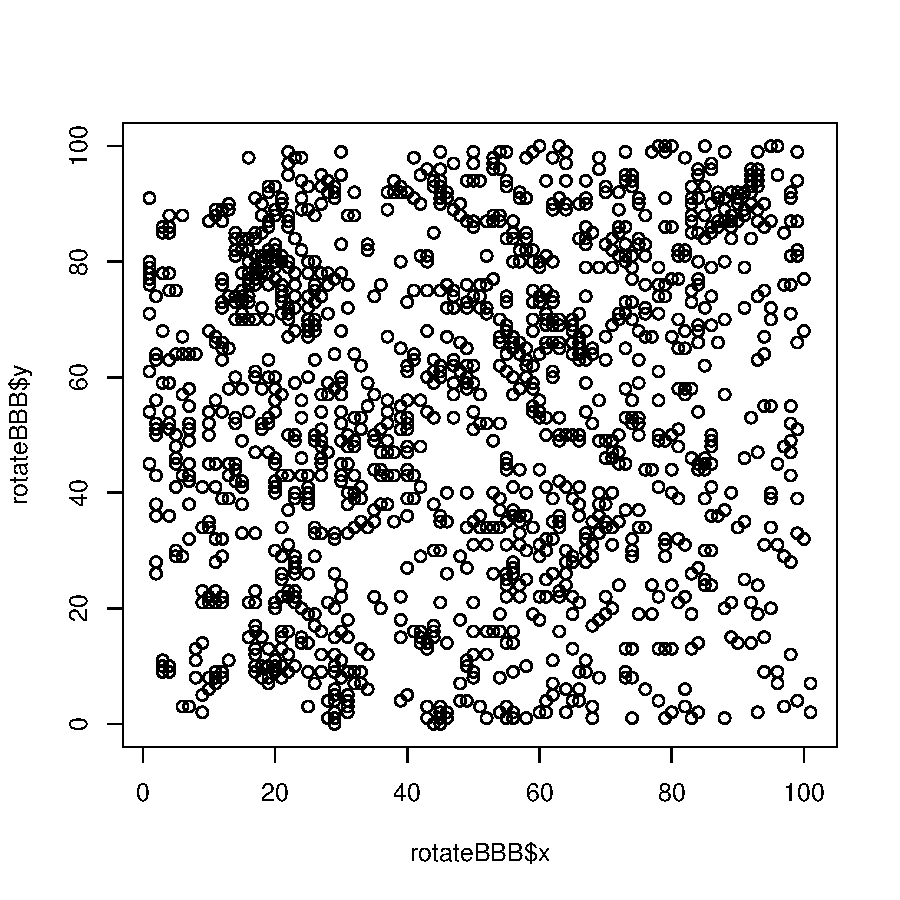
\includegraphics{SubPlotBoundaries-002}

Ok, so we know the plot is 100x100, and we know the subplot file originally used had the important columns: "Subplot", "POINT\_X", and "POINT\_Y". So, we need to replicate that. Let's build all of the corners, then look in the middle for a subplot identity.

\begin{Schunk}
\begin{Sinput}
> ## A function to get all possible values of x
> getSubplotCoords <- function(corners, increment=25){
+   xcount <- corners[1]+increment
+   xmax <- corners[2]
+   response <- corners[1]
+ 
+   while(xcount < xmax){
+     response <- c(response, xcount)
+     xcount <- xcount+increment
+   }
+   response <- c(response, xcount) ## do last one, so it encompasses all points
+   return(response)
+ }
> ## get coords
>   xcoords <- getSubplotCoords(corners[1:2])
>   ycoords <- getSubplotCoords(corners[3:4])
> ##make sure the values are right...
>   xcoords
\end{Sinput}
\begin{Soutput}
[1]   1  26  51  76 101
\end{Soutput}
\begin{Sinput}
>   ycoords
\end{Sinput}
\begin{Soutput}
[1]   0  25  50  75 100
\end{Soutput}
\begin{Sinput}
> buildBoxes <- function(x, y){
+ 
+   ## get the number of subplots by row and column
+   numxbox <- length(x)-1
+   numybox <- length(y)-1
+   ## total number of subplots needed
+   boxes <- numxbox * numybox
+   ## number of rows for corners
+   rows <- boxes * 4
+ 
+   ## rep x appropriately
+   pointx <- sort(c(rep(x[2:numxbox], 4),
+                    rep(x[1], 2),
+                    rep(x[numxbox+1], 2)))
+ 
+   ## dummy value for pointy
+   pointy <- vector()
+   ## get pointy values, varied appropriately to match the x vals
+   for(i in 1:numybox){
+     pointy <- c(pointy,rep(c(y[i], y[i+1]),numxbox*2))
+   }
+ 
+   response <- data.frame(POINT_X=pointx,
+                          POINT_Y=pointy,
+                          Subplot=sort(rep(1:(rows/4), 4)),
+                          stringsAsFactors = FALSE)
+   ##for each X, up to the second to last one...
+ 
+   return(response)
+ }
> bbbpipoSubs <- buildBoxes(xcoords, ycoords)
> plot(rotateBBB$x, rotateBBB$y)
> points(bbbpipoSubs$POINT_X, bbbpipoSubs$POINT_Y, col="red", pch="X")
\end{Sinput}
\end{Schunk}
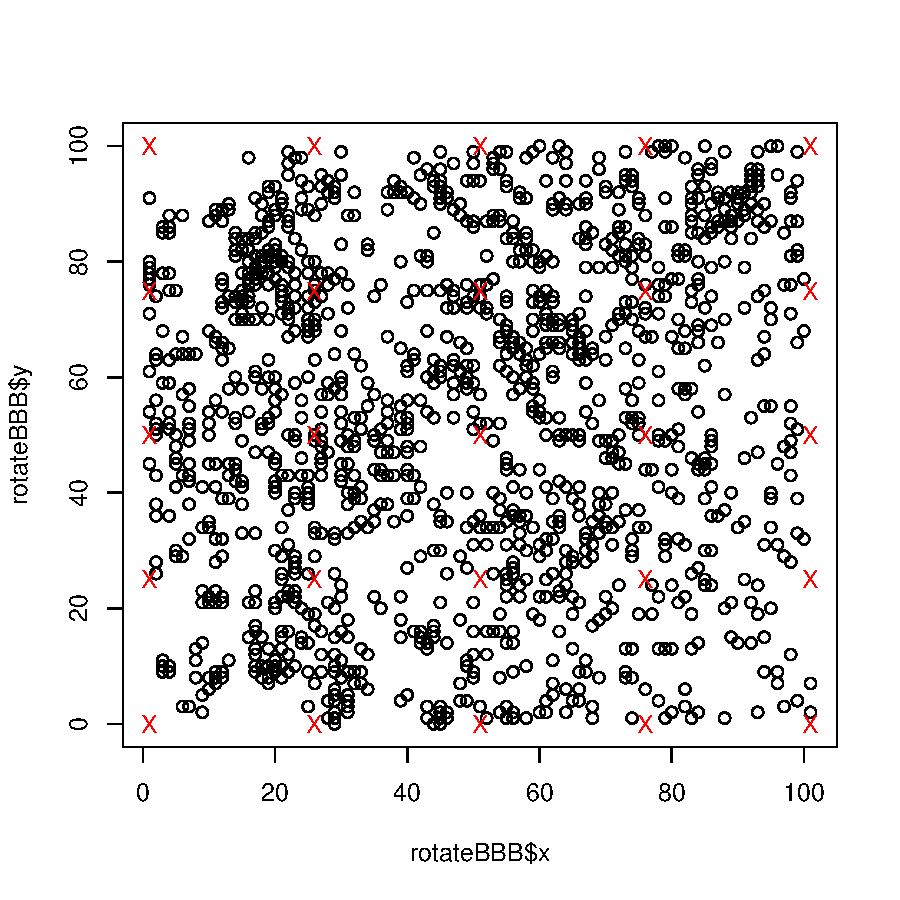
\includegraphics{SubPlotBoundaries-003}

The last thing we need to do is to make sure that our Subplots in the real data are assigned correctly, because our rotation may mean that our arbitrary Subplot numbers assigned in buildBoxes is incorrect. Definitely means they were incorrect. Those were just placeholders.

We can do that by subsetting for each of our current subplot identifiers in buildBoxes and assigning the correct one.

\begin{Schunk}
\begin{Sinput}
> assignSubplots <- function(df, subplotdf){
+   subplots <- unique(subplotdf$Subplot)
+ 
+ 
+   ## for each subplot ID currently (1:16)
+   for(i in 1:length(subplots)){
+     ## only get the subplots with that identity
+     reducedSub <- subplotdf[subplotdf$Subplot==subplots[i],]
+     ## get the corners
+     minx <- min(reducedSub$POINT_X)
+     maxx <- max(reducedSub$POINT_X)
+     miny <- min(reducedSub$POINT_Y)
+     maxy <- max(reducedSub$POINT_Y)
+ 
+     ## get the reduced other Df
+     reducedDf <- df[df$x > minx &
+                       df$x < maxx &
+                       df$y > miny &
+                       df$y < maxy,]
+ 
+     ## if there's more than one subplot in the designation...
+     if(length(unique(reducedDf$subplot))>1){
+       uniquesubs <- unique(reducedDf$subplot)
+       #print(paste("Unique SubPlots:", uniquesubs))
+         ## set the first record as a possible winner
+         winner <- 0
+         counts <- vector()
+       for(j in 1:length(uniquesubs)){
+         ##first time, winner=0, should eval to true
+         counted <- nrow(reducedDf[reducedDf$subplot==uniquesubs[j],])
+         if(counted > winner){
+           winner <- counted
+           majority <- uniquesubs[j]
+         }
+         counts <- c(counts, counted)
+       }
+       subplotdf[subplotdf$Subplot==subplots[i], "newsub"] <- majority
+       #print(counts)
+     } else{
+       ## there's only one subplot, we're golden.
+       subplotdf[subplotdf$Subplot==subplots[i],"newsub"] <- unique(
+                                                             reducedDf$subplot)
+     }
+   }
+   subplotdf$Subplot <- subplotdf$newsub
+   final <- subplotdf[, c("POINT_X", "POINT_Y", "Subplot")]
+   return(final)
+ }
> ## look at results
> finalsubplots <- assignSubplots(rotateBBB, bbbpipoSubs)
> head(finalsubplots)
\end{Sinput}
\begin{Soutput}
  POINT_X POINT_Y Subplot
1       1       0       4
2       1      25       4
3      26       0       4
4      26      25       4
5      26       0       8
6      26      25       8
\end{Soutput}
\begin{Sinput}
> tail(finalsubplots)
\end{Sinput}
\begin{Soutput}
   POINT_X POINT_Y Subplot
59      76      75       9
60      76     100       9
61      76      75      13
62      76     100      13
63     101      75      13
64     101     100      13
\end{Soutput}
\begin{Sinput}
> ##write.csv(finalsubplots, file="bbbpipo-subplots.csv")
> 
\end{Sinput}
\end{Schunk}

Okay, so I think we have all of the parts that we need to run traploc. Let's load up that function and try it out.

\begin{Schunk}
\begin{Sinput}
> ## unedited, from traploc.R
> ##
> 
> trap_UTM <- function(filename,subplots,site,bearing=0,plotcorns=list(F)) {
+ # filename = the filename with directory path for the csv of the GIS attribute
+ # table; subplots = the subplots that have the traps in them site = the site
+ # name; bearing = the approx bearing of the site #### NOT WORKING FOR OTHERS
+ # THAN NORTH!! ; plotcorns = a list of a logical toggle to print a map of the
+ # seed trap locations and the path/filename of the figure
+ 
+ ### STILL TO DO:
+ #   -- fix for a non-northfacing plot
+ #   -- make a function for find the directional corners based on the bearing
+ #   -- do the geometry for adding the offset
+ #   -- look through all the files in the "Seedling_reloc_details" folder to add
+ #        irregularities to the each plot (note: SeedlingPlotInfo.xls matches up
+ #        the old names to the new)
+ 
+   # save the default options, then set stringsAsFactors to False
+ 	holdopt <- options()["stringsAsFactors"]; options(stringsAsFactors=F)
+ 
+ 	# import the polygon corners
+ 	pcor <- read.csv(file=filename,header=T,as.is=T)
+ 
+ 	# get the subplot length
+ 	spl <- length(subplots)
+ 
+ 	## set up response data.frame
+ 	outdat <- data.frame(
+ 	  ID=rep("none",9*spl),
+ 	  PLOT_NAME=rep(site,9*spl),
+ 	  SUBPLOT=rep(subplots,each=9),
+ 	  TRAP=rep(1:9,spl),
+ 	  XCoord=rep(-99.99,9*spl),
+ 	  YCoord=rep(-99.99,9*spl))
+ 
+ 	##make the ID column
+ 	outdat$ID <- paste(outdat$PLOT_NAME,outdat$SUBPLOT,outdat$TRAP,sep="-")
+ 
+ 	##set up other output variables
+     allcns <- data.frame()
+     allposc <- c()
+ 
+ 
+     ##for each subplot
+ 	  for (i in subplots) {
+ 	    ## extract the subplot corners from GIS output file
+ 		  cns <- pcor[which(pcor$Subplot==i),c("POINT_X","POINT_Y")]
+ 		  colnames(cns) <- c("x","y")
+ 
+ 		   # get rid of the duplicated point --
+ 		   # the GIS polygon repeats the first and
+ 		   # last point
+ 		  cns <- cns[!duplicated(cns),]
+ 		  allcns <- rbind(allcns,cns)
+ 
+ 		  # find the minimum and maximum corner points
+ 		  minx <- min(cns$x)
+ 		  miny <- min(cns$y)
+ 		  maxx <- max(cns$x)
+ 		  maxy <- max(cns$y)
+ 
+ 		# make a vector that knows the corners -- CHANGE THIS IF bearing !=0
+ 		posc <- rep(0,4)
+ 
+ 		##find each corner, sw=swc, etc.
+ 		  swc <- which(cns$x < minx+1 & cns$y < miny+1)
+ 		  posc[swc] <- "swc"
+ 
+ 		  sec <- which(cns$x > cns$x[swc] & cns$y < miny+1)
+ 		  posc[sec] <- "sec"
+ 
+ 		  nwc <- which(cns$x < minx+1 & cns$y > cns$y[swc])
+ 		  posc[nwc] <- "nwc"
+ 
+ 		  nec <- which(cns$x > cns$x[swc] & cns$y > cns$y[swc])
+ 		  posc[nec] <- "nec"
+ 
+ 		  allposc <- c(allposc,posc)
+ 
+ 		### OFFSETS need to be CHANGED if bearing != 0
+ 		# trap 1: swc corner
+ 		# ang <- # find angle of line and muliply cos/sin the offset
+ 		outdat$XCoord[
+ 		  which(outdat$SUBPLOT==i & outdat$TRAP==1)] <- cns$x[
+             which(posc=="swc")]-0.25
+ 		outdat$YCoord[
+ 		  which(outdat$SUBPLOT==i & outdat$TRAP==1)] <- cns$y[
+             which(posc=="swc")]-0.25
+ 
+ 		# trap 2: side between swc & nwc
+ 		outdat$XCoord[
+ 		  which(outdat$SUBPLOT==i & outdat$TRAP==2)] <- mean(c(
+             cns$x[which(posc=="swc")],
+             cns$x[which(posc=="nwc")])
+             )-0.25
+ 		outdat$YCoord[
+ 		  which(outdat$SUBPLOT==i & outdat$TRAP==2)] <- mean(c(
+     		    cns$y[which(posc=="swc")],
+     		    cns$y[which(posc=="nwc")])
+     		    )
+ 
+ 		# trap 3: nwc corner
+ 		outdat$XCoord[
+ 		  which(outdat$SUBPLOT==i & outdat$TRAP==3)] <- cns$x[
+             which(posc=="nwc")]-0.25
+ 		outdat$YCoord[
+ 		  which(outdat$SUBPLOT==i & outdat$TRAP==3)] <- cns$y[
+             which(posc=="nwc")]+0.25
+ 
+ 		# trap 4: side between swc and sec
+ 		outdat$XCoord[
+ 		  which(outdat$SUBPLOT==i & outdat$TRAP==4)] <- mean(c(
+   		    cns$x[which(posc=="swc")],
+   		    cns$x[which(posc=="sec")])
+   		    )
+ 		outdat$YCoord[
+ 		  which(outdat$SUBPLOT==i & outdat$TRAP==4)] <- mean(c(
+     		    cns$y[which(posc=="swc")],
+     		    cns$y[which(posc=="sec")])
+     		    )-0.25
+ 
+ 		# trap 5: center
+ 		outdat$XCoord[
+ 		  which(outdat$SUBPLOT==i & outdat$TRAP==5)] <- mean(c(
+     		    cns$x[which(posc=="swc")],
+     		    cns$x[which(posc=="nec")])
+     		    )
+ 		outdat$YCoord[
+ 		  which(outdat$SUBPLOT==i & outdat$TRAP==5)] <- mean(c(
+     		    cns$y[which(posc=="swc")],
+     		    cns$y[which(posc=="nec")])
+     		    )
+ 
+ 		# trap 6: side between nwc and nec
+ 		outdat$XCoord[
+ 		  which(outdat$SUBPLOT==i & outdat$TRAP==6)] <- mean(c(
+   		    cns$x[which(posc=="nwc")],
+   		    cns$x[which(posc=="nec")])
+   		    )
+ 		outdat$YCoord[
+ 		  which(outdat$SUBPLOT==i & outdat$TRAP==6)] <- mean(c(
+     		    cns$y[which(posc=="nwc")],
+     		    cns$y[which(posc=="nec")])
+     		    )+0.25
+ 
+ 		# trap 7: sec corner
+ 		outdat$XCoord[
+ 		  which(outdat$SUBPLOT==i & outdat$TRAP==7)] <- cns$x[
+     		    which(posc=="sec")]
+     	      +0.25
+ 		outdat$YCoord[
+ 		  which(outdat$SUBPLOT==i & outdat$TRAP==7)] <- cns$y[
+             which(posc=="sec")]
+             -switch(site,
+             "PGABMA"=ifelse(i==6,1.8,0.25),0.25)
+ 
+ 		# trap 8: side between sec and nec
+ 		outdat$XCoord[
+ 		  which(outdat$SUBPLOT==i & outdat$TRAP==8)] <- mean(c(
+     		    cns$x[which(posc=="sec")],
+     		    cns$x[which(posc=="nec")])
+     		    )+0.25
+ 		outdat$YCoord[
+ 		  which(outdat$SUBPLOT==i & outdat$TRAP==8)] <- mean(c(
+     		    cns$y[which(posc=="sec")],
+     		    cns$y[which(posc=="nec")])
+     		    )
+ 
+ 		# trap 9: nec corner
+ 		outdat$XCoord[
+ 		  which(outdat$SUBPLOT==i & outdat$TRAP==9)] <- cns$x[
+     		    which(posc=="nec")]
+     		    +0.25
+ 		outdat$YCoord[
+ 		  which(outdat$SUBPLOT==i & outdat$TRAP==9)] <- cns$y[
+             which(posc=="nec")]
+             +0.25
+ 
+ 	}  # end for loop thru subplots
+ 	rm(i)
+ 
+ 	if (plotcorns[[1]]) {   # make a figure of the seed corners if T
+ 		png(filename=plotcorns[[2]],width=960,height=960)
+ 			plot(allcns$x,
+ 			     allcns$y,
+ 			     pch=2,
+ 			     col="white",
+ 			     main=site)
+ 			text(allcns$x,
+ 			     allcns$y,
+ 			     labels=allposc,
+ 			     cex=0.5)
+ 
+ 			subtrap <- paste(outdat$SUBPLOT,outdat$TRAP,sep="-")
+ 			text(outdat$XCoord,
+ 			     outdat$YCoord,
+ 			     labels=subtrap,
+ 			     cex=0.5)
+ 		dev.off()
+ 	}
+ 
+ 	options(stringsAsFactors=holdopt)   # return the options to the original
+ 
+ 	return(outdat)
+ }  # end function
> 
> 
> 
\end{Sinput}
\end{Schunk}

Okay, and just to keep it need and clean, let's get the trap coordinates using this function, and plot them overtop of our map.

\begin{Schunk}
\begin{Sinput}
> trapcoords <- trap_UTM(
+   filename="../data/BBBPIPO_subpolygon_corners.csv",
+   subplots=c(6,11),
+   site="BBBPIPO",
+   bearing=0,
+   plotcorns=list(T,paste("../data/","BBBPIPO","_traps.png",sep="")))
> plot(rotateBBB$x, rotateBBB$y, pch=".")
> points(trapcoords$XCoord, trapcoords$YCoord, col="red")
\end{Sinput}
\end{Schunk}
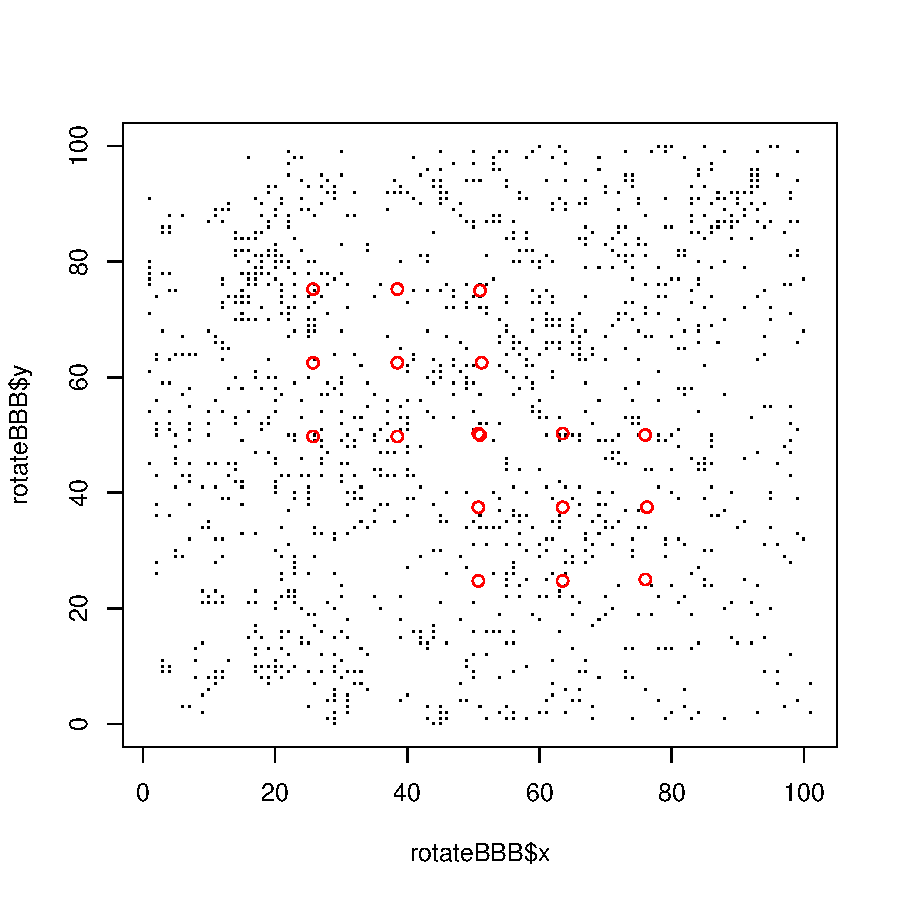
\includegraphics{SubPlotBoundaries-006}

And there we have it. Now, we just need to wrap everything up in a pretty package, and we can execute it more efficiently for the other plots. Then we can take our seedtrap locations and use disperseR to calculate seed dispersal. Finally.


\end{document}
